\documentclass[12pt, oneside]{article}

\usepackage[letterpaper, scale=0.89, centering]{geometry}
\usepackage{fancyhdr}
\setlength{\parindent}{0em}
\setlength{\parskip}{1em}

\usepackage{tikz}
\usetikzlibrary{automata,positioning,arrows}

\pagestyle{fancy}
\fancyhf{}
\renewcommand{\headrulewidth}{0pt}
\rfoot{\href{https://creativecommons.org/licenses/by-nc-sa/2.0/}{CC BY-NC-SA 2.0} Version \today~(\thepage)}

\usepackage{amssymb,amsmath,pifont,amsfonts,comment,enumerate,enumitem}
\usepackage{currfile,xstring,hyperref,tabularx,graphicx,wasysym}
\usepackage[labelformat=empty]{caption}
\usepackage{xcolor}
\usepackage{multicol,multirow,array,listings,tabularx,lastpage,textcomp,booktabs}

\lstnewenvironment{algorithm}[1][] {   
    \lstset{ mathescape=true,
        frame=tB,
        numbers=left, 
        numberstyle=\tiny,
        basicstyle=\rmfamily\scriptsize, 
        keywordstyle=\color{black}\bfseries,
        keywords={,procedure, div, for, to, input, output, return, datatype, function, in, if, else, foreach, while, begin, end, }
        numbers=left,
        xleftmargin=.04\textwidth,
        #1
    }
}
{}

\newcommand\abs[1]{\lvert~#1~\rvert}
\newcommand{\st}{\mid}

\newcommand{\cmark}{\ding{51}}
\newcommand{\xmark}{\ding{55}}
 
\begin{document}
\begin{flushright}
    \StrBefore{\currfilename}{.}
\end{flushright} \section*{Week2 monday}


{\bf Review}: Formal definition of DFA: $M = (Q, \Sigma, \delta, q_0, F)$ 

\begin{center}
\begin{multicols}{2}
\begin{itemize}
\setlength{\itemsep}{2pt}
\item Finite set of states $Q$
\item Alphabet $\Sigma$
\item Transition function $\delta$
\item Start state $q_0$
\item Accept (final) states $F$
\end{itemize}
\end{multicols}
\end{center}
Quick check: In the state diagram of $M$, how many outgoing arrows are there from each state?



{\bf Note}: We'll see a new kind of finite automaton. It will be helpful to distinguish it from the
machines we've been talking about so we'll use {\bf Deterministic Finite Automaton} (DFA) to refer to the machines 
from Section 1.1.

$M = ( \{ q0, q1, q2\}, \{a,b\}, \delta, q0, \{q0\} )$ 
where $\delta$ is  (rows labelled by states
and columns labelled by symbols):
\begin{center}
\begin{tabular}{c|cc}
$\delta$ & $a$ & $b$ \\
\hline
$q0$ & $q1$ & $q1$ \\
$q1$ & $q2$ & $q2$ \\
$q2$ & $q0$ & $q0$ \\
\end{tabular}
\end{center}

The state diagram for $M$ is 

\vfill


Give two examples of strings that are accepted by $M$ and two examples of strings that are rejected by $M$:

\vfill


A regular expression describing $L(M)$ is


\vfill 

A state diagram for a finite automaton recognizing
$$\{w \mid w~\text{is a string over $\{a,b\}$ whose length is not a multiple of $3$} \}$$

\vfill

Extra example: Let $n$ be an arbitrary positive integer. What is a formal definition for a finite automaton recognizing
\[
\{w \mid w~\text{is a string over $\{0,1\}$ whose length is not a multiple of $n$} \}?
\]

\newpage

Consider the alphabet $\Sigma_1 = \{0,1\}$.

A state diagram for a finite automaton that recognizes $\{w \mid w~\text{contains at most two $1$'s} \}$ is

\vspace{70pt}

A state diagram for a finite automaton that recognizes $\{w \mid w~\text{contains more than two $1$'s} \}$ is

\vspace{70pt}


\textbf{Strategy}: Add ``labels" for states in the state diagram, 
e.g. ``have not seen any of desired pattern yet'' or
``sink state''. Then, we can use the analysis of the roles of the states in the 
state diagram to work towards a description of the language recognized
by the finite automaton.


Or: decompose the language to a simpler one 
that we already know how to recognize with a DFA or NFA.


Textbook Exercise 1.14: 
Suppose $A$ is a language over an alphabet $\Sigma$. 
If there is a DFA $M$ such that $L(M) = A$ then there is another DFA, let's call it $M'$, such that 
$L(M') = \overline{A}$, the complement of $A$, defined as $\{ w \in \Sigma^* \mid w \notin A \}$.


{\bf Proof idea}:


\vfill
A useful bit of terminology: the {\bf iterated transition function} of a finite automaton
$M = (Q, \Sigma, \delta, q_0, F)$ is defined recursively by
\[
\delta^* (~(q,w)~) 
=\begin{cases}
q  \qquad &\text{if $q \in Q, w = \varepsilon$} \\
\delta( ~(q,a)~) \qquad &\text{if $q \in Q$, $w = a \in \Sigma$ } \\
\delta(~(\delta^*(~(q,u)~), a) ~) \qquad &\text{if $q \in Q$, $w = ua$ where $u \in  \Sigma^*$ and $a \in \Sigma$}
\end{cases}
\]

Using  this terminology, $M$ accepts a string $w$ over $\Sigma$ if and only if $\delta^*( ~(q_0,w)~) \in F$.


{\bf Proof}: 
\vfill


 \vfill
\section*{Week2 wednesday}


\begin{center}
\begin{tabular}{|ll|}
\hline
\multicolumn{2}{|l|}{{\bf Nondeterministic finite automaton}  (Sipser Page 53) Given as $M = (Q, \Sigma, \delta, q_0, F)$}\\
& \\
Finite set of states $Q$  & Can  be labelled by any collection  of distinct names. Default: $q0, q1, \ldots$  \\
Alphabet $\Sigma$ &  Each input to the automaton is a string over  $\Sigma$. \\
Arrow labels $\Sigma_\varepsilon$ &  $\Sigma_\varepsilon = \Sigma \cup \{ \varepsilon\}$. \\
&  Arrows 
in the state diagram are labelled either by symbols from $\Sigma$ or by $\varepsilon$ \\
Transition function $\delta$  & $\delta: Q \times \Sigma_{\varepsilon} \to \mathcal{P}(Q)$
gives the {\bf set of possible next states} for a transition \\
&  from the current state upon reading a symbol or spontaneously moving.\\
Start state $q_0$ & Element of $Q$.  Each computation of the machine starts at the  start  state.\\
Accept (final) states $F$ & $F \subseteq  Q$.\\
& \\
\multicolumn{2}{|p{\textwidth}|}{$M$ accepts the input string $w \in \Sigma^*$ if and only if {\bf there is} a computation of $M$ on 
$w$ that processes the whole string and ends in an
accept state.}\\
\hline
\end{tabular}
\end{center}

The formal definition of the NFA over $\{0,1\}$ given by this state diagram is: 

\includegraphics[width=2in]{Lect4NFA1.png}

The language over $\{0,1\}$ recognized by this NFA is:

\vspace{70pt}

Change the transition function to get a different NFA which accepts
the empty string (and potentially other strings too).


\newpage

The state diagram of an NFA over $\{a,b\}$ is below.  The formal definition of this NFA is:

\vspace{-30pt}

\includegraphics[width=2.5in]{Lect5NFA1.png}


Suppose $A_1, A_2$ are languages over an alphabet $\Sigma$.
{\bf Claim:} if there is a NFA $N_1$ such that $L(N_1) = A_1$ and 
NFA $N_2$ such that $L(N_2) = A_2$, then there is another NFA, let's call it $N$, such that 
$L(N) = A_1 \cup A_2$.

{\bf Proof idea}: Use nondeterminism to choose which of $N_1$, $N_2$ to run.

\vfill
\begin{comment}
    Draw schematic
\end{comment}

{\bf Formal construction}: Let 
$N_1 = (Q_1, \Sigma, \delta_1, q_1, F_1)$ and $N_2 = (Q_2, \Sigma, \delta_2,q_2, F_2)$
and assume $Q_1 \cap Q_2 = \emptyset$ and that $q_0 \notin Q_1 \cup Q_2$.
Construct $N = (Q, \Sigma, \delta, q_0, F_1 \cup F_2)$ where
\begin{itemize}
    \item $Q = $
    \item $\delta: Q \times \Sigma_\varepsilon \to \mathcal{P}(Q)$ is defined by, for $q \in Q$ and $x \in \Sigma_{\varepsilon}$:
        \[
            \phantom{\delta((q,x))=\begin{cases}  \delta_1 ((q,x)) &\qquad\text{if } q\in Q_1 \\ \delta_2 ((q,x)) &\qquad\text{if } q\in Q_2 \\ \{q1,q2\} &\qquad\text{if } q = q_0, x = \varepsilon \\ \emptyset\text{if } q= q_0, x \neq \varepsilon \end{cases}}
        \]
\end{itemize}


\vfill
{\it Proof of correctness would prove that $L(N) = A_1 \cup A_2$ by considering
an arbitrary string accepted by $N$, tracing an accepting computation of $N$ on it, and using 
that trace to prove the string is in at least one of $A_1$, $A_2$; then, taking an arbitrary 
string in $A_1 \cup A_2$ and proving that it is accepted by $N$. Details left for extra practice.}
 \vfill
\section*{Week2 friday}


{\bf Review}: The language recognized by the NFA over $\{a,b\}$ with state diagram


    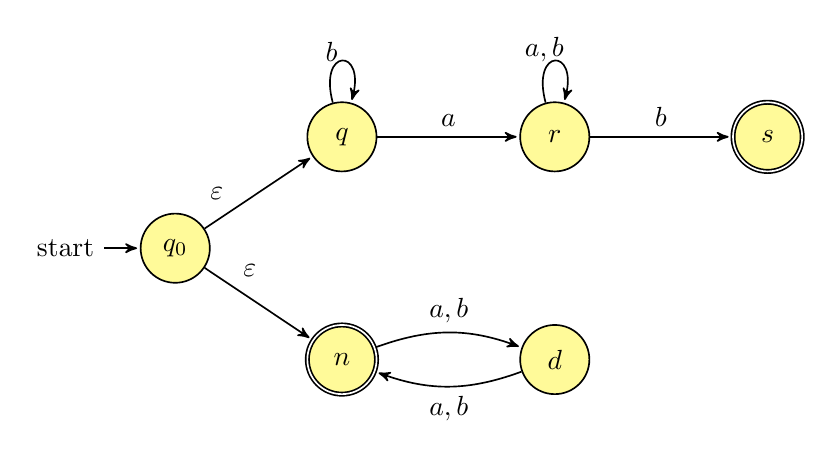
\begin{tikzpicture}[->,>=stealth',shorten >=1pt, auto, node distance=2cm, semithick]
    \tikzstyle{every state}=[text=black, fill=yellow!40]
    
    \node[initial,state] (q0)          {$q_0$};
    \node[state]         (q) [above right of=q0, xshift=20pt] {$q$};
    \node[state]         (r) [right of=q, xshift=20pt] {$r$};
    \node[state, accepting]         (s) [right of=r, xshift=20pt] {$s$};
    \node[state, accepting]         (n) [below right of=q0, xshift=20pt] {$n$};
    \node[state]         (d) [right of=n, xshift=20pt] {$d$};
    
    \path (q0) edge  [bend left=0, near start] node {$\varepsilon$} (q)
            edge [bend right=0, near start] node {$\varepsilon$} (n)
        (q) edge [bend left=0] node {$a$} (r)
            edge [loop above, near start] node {$b$} (q)
        (r) edge [bend left=0] node {$b$} (s)
            edge [loop above, near start] node {$a,b$} (r)
        (n) edge [bend left=20] node {$a,b$} (d)
        (d) edge [bend left=20] node {$a,b$} (n)
    ;
    \end{tikzpicture}
is:


\vfill

So far, we know: 
\begin{itemize}
\item The collection of languages that are each recognizable by a 
DFA is {\bf closed} under complementation.

{\it Could we do the same construction with NFA?}

\vspace{100pt}

\item The collection of languages that are each recognizable by a 
NFA is {\bf closed} under complementation.

{\it Could we do the same construction with DFA?}

\vspace{100pt}

\end{itemize}


\newpage

\vspace{50pt}

Happily, though, an analogous claim is true!

Suppose $A_1, A_2$ are languages over an alphabet $\Sigma$.
{\bf Claim:} if there is a DFA $M_1$ such that $L(M_1) = A_1$ and 
DFA $M_2$ such that $L(M_2) = A_2$, then there is another DFA, let's call it $M$, such that 
$L(M) = A_1 \cup A_2$. {\it Theorem 1.25 in Sipser, page 45}
    
    {\bf Proof idea}:
    
    
    {\bf Formal construction}: 
    
    \vfill

    
    {\bf Example}:  When $A_1 = \{w \mid w~\text{has an $a$ and ends in $b$} \}$ and 
    $A_2 = \{ w \mid w~\text{is of even length} \}$.
    
    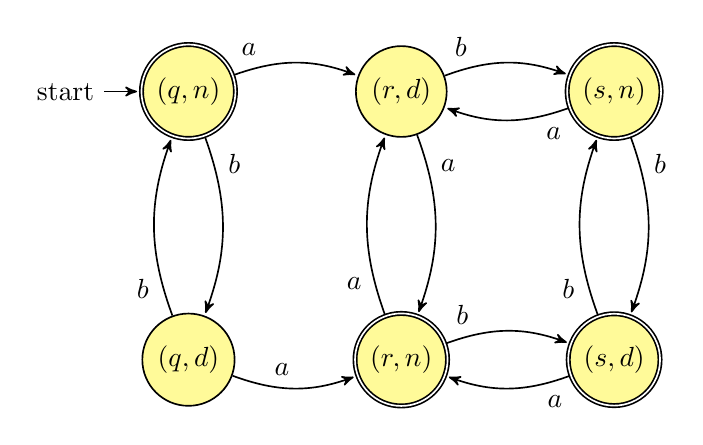
\begin{tikzpicture}[->,>=stealth',shorten >=1pt, auto, node distance=2cm, semithick]
        \tikzstyle{every state}=[text=black, fill=yellow!40]
        
        \node[initial,state,accepting] (qn)          {$(q,n)$};
        \node[state]         (qd) [below of=qn, yshift=-40pt] {$(q,d)$};
        \node[state]         (rd) [right of=qn, xshift=20pt] {$(r,d)$};
        \node[state,accepting]         (rn) [right of=qd, xshift=20pt] {$(r,n)$};
        \node[state,accepting]         (sn) [right of=rd, xshift=20pt] {$(s,n)$};
        \node[state,accepting]         (sd) [right of=rn, xshift=20pt] {$(s,d)$};
        
        \path (qn) edge  [bend left=20, near start] node {$b$} (qd)
                edge [bend left=20, near start] node {$a$} (rd)
            (qd) edge [bend left=20, near start] node {$b$} (qn)
                edge [bend right=20, near start] node {$a$} (rn)
            (rn) edge [bend left=20, near start] node {$a$} (rd)
                edge [bend left=20, near start] node {$b$} (sd)
            (rd) edge [bend left=20, near start] node {$a$} (rn)
                edge [bend left=20, near start] node {$b$} (sn)
            (sn) edge [bend left=20, near start] node {$a$} (rd)
                edge [bend left=20, near start] node {$b$} (sd)
            (sd) edge [bend left=20, near start] node {$a$} (rn)
                edge [bend left=20, near start] node {$b$} (sn)
        ;
        \end{tikzpicture}
    
    \newpage
    
    Suppose $A_1, A_2$ are languages over an alphabet $\Sigma$.
    {\bf Claim:} if there is a DFA $M_1$ such that $L(M_1) = A_1$ and 
    DFA $M_2$ such that $L(M_2) = A_2$, then there is another DFA, let's call it $M$, such that 
    $L(M) = A_1 \cap A_2$.  {\it Footnote to Sipser Theorem 1.25, page 46}
    
    {\bf Proof idea}:
    
    
    {\bf Formal construction}: 
    
    \vspace{70pt}


    
 \vfill
\section*{Week0 friday}


The CSE 105 vocabulary and notation build on discrete
math and introduction to proofs classes.  Some of the conventions may 
be a bit different from what you saw before so we'll draw your attention to them.

For consistency, we will use the notation from this class' textbook\footnote{Page references are to 
the 3rd edition of Sipser's Introduction to the Theory of Computation,
available through various sources for approximately \$30. You may be able to 
opt in to purchase a digital copy through Canvas. Copies of the book are also available 
for those who can't access the book
to borrow from the course instructor, while supplies last (minnes@ucsd.edu)}.

These definitions are on pages 3, 4, 6, 13, 14, 53.

\begin{center}
    \begin{tabular}{|p{2.6in}cp{3.5in}|}
    \hline 
    {\bf Term} & {\bf Typical symbol} & {\bf Meaning} \\
     & or {\bf Notation} & \\
    \hline
    && \\
    Alphabet & $\Sigma$, $\Gamma$ & A non-empty finite set	 \\
    Symbol over $\Sigma$  & $\sigma$, $b$, $x$ & An element of the alphabet $\Sigma$\\ 
    String over $\Sigma$  &	$u$, $v$, $w$ & A finite list of symbols from $\Sigma$\\
    (The) empty string &$\varepsilon$ & The (only) string of length $0$\\
    The set of all strings over $\Sigma$ & $\Sigma^*$ & The collection of all possible strings formed from symbols from $\Sigma$ \\ 
    (Some) language over $\Sigma$& $L$ & (Some) set of strings over $\Sigma$ \\ 
    (The) empty language &$\emptyset$ & The empty set, i.e. the set that has no strings (and no other elements either)\\
    && \\
    \hline
    && \\
    The power set of a set $X$ &$\mathcal{P}(X)$ & The set of all subsets of $X$ \\
    (The set of) natural numbers &$\mathcal{N}$ & The set of positive integers \\ 
    (Some) finite set & & The empty set or a set whose distinct elements can be counted by a natural number\\
    (Some) infinite set & & A set that is not finite.\\ 
    &&\\
    \hline
    && \\
    Reverse of a string $w$ & $w^\mathcal{R}$  & write $w$  in  the opposite order, if $w = w_1 \cdots  w_n$ then $w^\mathcal{R} = w_n \cdots  w_1$. Note: $\varepsilon^\mathcal{R} = \varepsilon$\\
    Concatenating strings $x$ and $y$ & $xy$ &  take $x = x_1 \cdots x_m$, $y=y_1 \cdots y_n$ and form $xy = x_1 \cdots x_m y_1 \cdots y_n$\\
    String $z$ is a substring of string $w$ & & there are strings $u,v$ such that $w = uzv$\\
    String $x$ is a prefix of string $y$ & & there is a string $z$ such that $y = xz$ \\
    String $x$ is a proper prefix of string $y$ & & $x$ is a prefix of $y$ and $x \neq y$\\
    && \\
    \hline
    &&\\
    Shortlex order, also known as string order over alphabet $\Sigma$ & & Order strings over  $\Sigma$ first 
    by length and then according to the dictionary order, assuming symbols in $\Sigma$  have an ordering\\ \hline
    \end{tabular}
\end{center}

\vfill
    
\newpage
Write out in words the meaning of the symbols below: 

\[
    \{ a, b, c\}
\]

\phantom{The set whose elements are $a$, $b$, and $c$}

\[
    | \{a, b, a \} | = 2
\]

\phantom{The number of elements in the set $\{a,b,a\}$ is $2$.}

\[
    | aba | = 3
\]

\phantom{The length of the string $aba$ is $3$.}

\begin{comment}

\[
    (a, 3, 2, b, b)
\]

\phantom{The $5$-tuple whose first components is $a$, second component 
is $3$, third component is $2$, fourth component is $b$, and fifth component is $b$.}
\end{comment}

{\it Circle the correct choice}:

A {\bf string} over an alphabet $\Sigma$ is \underline{~~an element of $\Sigma^*$ ~~ OR ~~ a subset of $\Sigma^*$}.
    
A {\bf language} over an alphabet $\Sigma$ is \underline{~~an element of $\Sigma^*$ ~~ OR ~~ a subset of $\Sigma^*$}.


With $\Sigma_1 = \{0,1\}$ and 
$\Sigma_2 = \{a,b,c,d,e,f,g,h,i,j,k,l,m,n,o,p,q,r,s,t,u,v,w,x,y,z\}$
and $\Gamma = \{0,1,x,y,z\}$

{\bf True} or {\bf False}: $\varepsilon \in \Sigma_1$

{\bf True} or {\bf False}: $\varepsilon$ is  a string over $\Sigma_1$

{\bf True} or {\bf False}: $\varepsilon$ is a language over $\Sigma_1$

{\bf True} or {\bf False}: $\varepsilon$ is a prefix of some string over  $\Sigma_1$

{\bf True} or {\bf False}: There is a string over $\Sigma_1$ that is a proper prefix of $\varepsilon$
    

The first five strings over $\Sigma_1$ in string order, using the ordering $0 <  1$: \vfill
    
The first five strings over $\Sigma_2$ in string order, using the usual alphabetical ordering for single letters: \vfill



 \vfill
\section*{Week1 monday}


Our motivation in studying sets of strings is that they can be used to encode problems.
To calibrate how difficult a problem is to solve, we describe how complicated the set of strings that encodes it is. 
How do we define sets of strings?


\vfill

How would you describe the language that has no elements at all?

\vfill

How would you describe the language that has all strings over $\{0,1\}$ as its elements?

\vfill

\newpage

**This definition was in the pre-class reading**
{\bf Definition 1.52}: A {\bf regular expression} over alphabet $\Sigma$
is a syntactic expression that can describe a language over $\Sigma$. The collection of all regular
expressions over $\Sigma$ is defined recursively:
\begin{itemize}
\item[] {\it Basis steps of recursive definition}
\begin{quote}    
    $a$ is a regular expression, for $a \in \Sigma$

    $\varepsilon$ is a regular expression

    $\emptyset$ is a regular expression
\end{quote}

\item[] {\it Recursive steps of recursive definition}
\begin{quote}
    $(R_1 \cup R_2)$ is a regular expression when $R_1$, $R_2$ are regular expressions 

    $(R_1 \circ R_2)$ is a regular expression when $R_1$, $R_2$ are regular expressions

    $(R_1^*)$ is a regular expression when $R_1$ is a regular expression 
\end{quote}
\end{itemize}
 

The {\it semantics} (or meaning) of the syntactic regular expression is the {\bf language
described by the regular expression}. The function that assigns a language to a regular expression
over $\Sigma$ is defined recursively, using familiar set operations:


\begin{itemize}
    \item[] {\it Basis steps of recursive definition}
    \begin{quote}    
        The language described by $a$, for $a \in \Sigma$, is $\{a\}$ and we write 
        $L(a) = \{a\}$
    
        The language described by $\varepsilon$ is $\{\varepsilon\}$ and we write 
        $L(\varepsilon) = \{ \varepsilon\}$
    
        The language described by $\emptyset$ is $\{\}$ and we write
        $L(\emptyset) = \emptyset$.
    \end{quote}
    
    \item[] {\it Recursive steps of recursive definition}
    \begin{quote}
        When $R_1$, $R_2$ are regular expressions, the language described by the regular
        expression $(R_1 \cup R_2)$ is the union of the languages described by $R_1$ and $R_2$, 
        and we write 
        $$L(~(R_1 \cup R_2)~) = L(R_1) \cup L(R_2) = \{ w \mid w \in L(R_1) \lor w \in L(R_2)\}$$
    
        When $R_1$, $R_2$ are regular expressions, the language described by the regular
        expression $(R_1 \circ R_2)$ is the concatenation of the languages described by $R_1$ and $R_2$, 
        and we write 
        $$L(~(R_1 \circ R_2)~) = L(R_1) \circ L(R_2) = \{ uv \mid u \in L(R_1) \land v \in L(R_2)\}$$
    
        When $R_1$ is a regular expression, the language described by the regular 
        expression $(R_1^*)$ is the {\bf Kleene star} of the language described by $R_1$ and we write
        $$L(~(R_1^*)~) = (~L(R_1)~)^* = \{ w_1 \cdots w_k \mid k \geq 0 \textrm{ and each } w_i \in L(R_1)\}$$
    \end{quote}
\end{itemize}
  
\newpage
For the following examples assume the alphabet is $\Sigma_1 =  \{0,1\}$:
    
The language described by the regular expression $0$ is $L(0) = \{ 0 \}$

The language described by the regular expression $1$ is $L(1)  = \{ 1 \}$

The language described by the regular expression $\varepsilon$ is $L(\varepsilon) = \{ \varepsilon  \}$

The language described by the regular expression $\emptyset$ is $L(\emptyset) = \emptyset$

The language described by the regular expression $(\Sigma_1 \Sigma_1 \Sigma_1)^*$ 
is $L(~(\Sigma_1 \Sigma_1 \Sigma_1)^*~) = $

\vfill

The language described by the regular expression $1^* \circ 1$ is $L(1^* \circ 1) = $

\vfill
 \vfill
\section*{Week1 wednesday}



{\bf Review}: Determine whether each statement below about regular expressions
over the alphabet $\{a,b,c\}$ is true or false:

\begin{comment}
True or False: \qquad 
   $a  \in L(~(a \cup b )~\cup c)$
\end{comment}

True or False: \qquad 
   $ab  \in L(~ (a \cup b)^*  ~)$
   
True or False: \qquad    
   $ba \in L( ~ a^* b^* ~)$
   
True or False: \qquad 
   $\varepsilon  \in L(a \cup b \cup c)$
   
True or False: \qquad 
   $\varepsilon  \in L(~ (a \cup b)^*  ~)$

True or False: \qquad 
   $\varepsilon \in L( ~ aa^* \cup bb^* ~)$

\vfill

{\it Shorthand and conventions} (Sipser pages 63-65)

\vspace{-20pt}

\begin{center}
    \begin{tabular}{|ll|}
    \hline
    & \\
    \multicolumn{2}{|l|}{Assuming $\Sigma$ is the alphabet, we use the following conventions}\\
    & \\
    $\Sigma$   & regular  expression describing language consisting of  all strings  of length  $1$ over $\Sigma$\\
    $*$ then $\circ$ then $\cup$   & precedence order, unless parentheses are used to change it\\
    $R_1R_2$ & shorthand  for  $R_1  \circ R_2$ (concatenation symbol is implicit) \\
    $R^+$ & shorthand for $R^* \circ R$ \\
    $R^k$ & shorthand for $R$ concatenated with itself $k$ times, where $k$ is a (specific) natural number\\
    & \\
    \hline
    \end{tabular}
\end{center}

\vfill 

{\bf Caution: many programming languages that support regular expressions build in functionality
that is more powerful than the ``pure'' definition of regular expressions given here. }

Regular expressions are everywhere (once you start looking for them).

Software tools and languages often have built-in support for regular expressions to describe
{\bf patterns} that we want to match (e.g. Excel/ Sheets, grep, Perl, python, Java, Ruby).

Under the hood, the first phase of {\bf compilers} is to transform the strings we write 
in code to tokens (keywords, operators, identifiers, literals). Compilers use regular expressions
to describe the sets of strings that can be used for each token type.

Next time: we'll start to see how to build machines that decide whether strings match the pattern
described by a regular expression.

\newpage

Practice with the regular expressions over $\{a,b\}$ below.

For example: Which regular expression(s) below describe a language that includes the string $a$ as an element?

$a^* b^*$ 

\vfill

$a(ba)^* b$

\vfill

$a^* \cup b^*$

\vfill

$(aaa)^*$

\vfill

$(\varepsilon \cup a) b$

\vfill \vfill
\section*{Week1 friday}



**This definition was in the pre-class reading**
A finite automaton (FA) is specified by  $M = (Q, \Sigma, \delta, q_0, F)$.
This $5$-tuple is called the {\bf formal definition} of the FA. The FA can also 
be represented by its state diagram: with nodes for the state, labelled edges specifying the 
transition function, and decorations on nodes denoting the start and accept states.

\begin{quote}
Finite set of states $Q$ can be labelled by any collection of distinct names. Often
we use default state labels $q0, q1, \ldots$ 
\end{quote}

\begin{quote}  
The alphabet $\Sigma$ determines the possible inputs to the automaton. 
Each input to the automaton is a string over  $\Sigma$, and the automaton ``processes'' the input
one symbol (or character) at a time.
\end{quote}

\begin{quote}
The transition function $\delta$ gives the next state of the automaton based on the current state of 
the machine and on the next input symbol.
\end{quote}

\begin{quote}
The start state $q_0$ is an element of $Q$.  Each computation of the machine starts at the  start  state.
\end{quote}

\begin{quote}
The accept (final) states $F$ form a subset of the states of the automaton, $F \subseteq  Q$. 
These states are used to flag if the machine accepts or rejects an input string.
\end{quote}


\begin{quote}
The computation of a machine on an input string is a sequence of states
in the machine,  starting with the start state, determined by transitions 
of the machine as it reads successive input symbols.
\end{quote}

\begin{quote}
The finite automaton $M$ accepts the given input string exactly when the computation of $M$ on the input string
ends in an accept state. $M$ rejects the given input string exactly when the computation of 
$M$ on the input string ends in a nonaccept state, that is, a state that is not in $F$.
\end{quote}

\begin{quote} 
The language of $M$, $L(M)$, is defined as the set of  all strings that are each accepted 
by the machine $M$. Each string that is rejected by $M$ is not in $L(M)$.
The language of $M$ is also called the language recognized by $M$.
\end{quote}   
   
What is {\bf finite} about all finite automata? (Select all that apply)
\begin{itemize}
   \item[$\square$] The size of the machine (number of states, number of arrows)
   \item[$\square$] The length of each computation of the machine
   \item[$\square$] The number of strings that are accepted by the machine
\end{itemize}
\newpage
  
\begin{figure}[h]
   \centering
   \includegraphics[width=3in]{Lect2DFA1.png} 
\end{figure}
   
The formal definition of this FA is
   
\vfill
\vfill
   

Classify each string $a, aa, ab, ba, bb, \varepsilon$ as accepted by the FA or rejected by the FA.  

{\it Why are these the only two options?}

\vspace{200pt}


The language recognized by this automaton is
  

\vfill

\newpage

\begin{figure}[h]
  \centering
  \includegraphics[width=3in]{Lect2DFA2.png} 
\end{figure}
   

The language recognized by this automaton is
  


\vfill

\hrule

\begin{figure}[h]
    \centering
    \includegraphics[width=3in]{Lect2DFA3.png} 
\end{figure}

The language recognized by this automaton is
  

\vfill \vfill
\end{document}